\documentclass[12pt]{article}
\usepackage[a4paper, total={6in, 8.5in}]{geometry}
\usepackage{graphicx}
\graphicspath{ {images/output/} }
\usepackage{amsmath}
\usepackage{minted}
\usepackage{multicol}
\usepackage{caption}
\usepackage[english]{babel}
\usepackage{placeins}
\usepackage{titling}


\begin{document}
\vspace*{\fill}
\begin{center}

    \emph{Heaven's Light is Our Guide} \\
    \textbf{Rajshahi University of Engineering and Technology} \\

    \begin{figure}[H]
        \centering
        
\includegraphics[scale=.34]{images/RUET_logo.png}
        \label{fig:ruet_logo}
    \end{figure}
    \vspace{5mm}

    \textbf{Course Code}\\
    ECE 2214\\
    \vspace{3mm}
    \textbf{Course Title}\\
    Numerical Methods and Discrete Mathematics Sessional

    \vspace{5mm}
    \textbf{Experiment Date:} {November 18, 2023},\\
    \textbf{Submission Date:} {December 2, 2023}\\

    \vspace{5mm}
    \textbf{Lab Report 10:} Implementing Secant method of root finding in MATLAB.

    \vspace{15mm}

    \begin{tabular}{c|c}
        \textbf{Submitted to} & \textbf{Submitted by} \\
        Md. Omaer Faruq Goni  & Md. Tajim An Noor     \\
        Lecturer              & Roll: 2010025         \\
        Dept of ECE, Ruet     &                       \\
    \end{tabular}

\end{center}
\vspace*{\fill}

\clearpage
\title{Finding root of nonlinear equation using Bisection Method.}
\author{}
\date{}
\maketitle

\section*{Introduction}
\subsection*{Bisection Method}
Bisection method is based on the fact that if $f(x)$ is real and continuous function, and for two initial guesses $a$ and $b$ brackets the root such that: $f(a)\times f(b)< 0$ then there exists at least one root between $a$ and $b$.\\\\
Root is obtained in Bisection method by successive halving the interval i.e. If $a$ and $b$ are two guesses then we compute new approximated root as:
\[c = \frac{(a+b)}{2}\]
Now we have following three different cases:
\begin{itemize}
    \item If $f(c)=0$ then the root is c.
    \item If $f(a)\times f(b)< 0$ then root lies between $a$ and $c$.
    \item If $f(a)\times f(c)> 0$ then root lies between $b$ and $c$.
\end{itemize}
And then the process is repeated until we find the root within desired accuracy.\cite{bisec}

\section*{Tools Used}
\begin{itemize}
    \item MATLAB R2021a - for writing and running code.
    \item MacTeX -\LaTeX  compiler.
    \item VS Code with \LaTeX workshop extension as a text editor.
\end{itemize}

\section*{Process}
\subsection*{Code for Bisection:}
\begin{minted}[breaklines, linenos]{matlab}
% Clearing Screen
clc

% Setting x as symbolic variable, in every string, x will be considered as a variable
syms x;

% Input Section
eqn = input('Enter non-linear equations: '); %input as normal string.
a = input('Enter first guess: ');
b = input('Enter second guess: ');
e = input('Tolerable error: '); %error margin

% Finding Functional Value
fa = eval(subs(eqn,x,a));
fb = eval(subs(eqn,x,b));

% Implementing Bisection Method
if fa*fb > 0 
    disp('Initial values does not create bracket around the root');
else
    c = (a+b)/2;
    fc = eval(subs(eqn,x,c));
    fprintf('\n\na\t\t\tb\t\t\tc\t\t\tf(c)\n');
    while abs(fc)>e
        fprintf('%f\t%f\t%f\t%f\n',a,b,c,fc);
        if fa*fc< 0
            b =c;
        else
            a =c;
        end
        c = (a+b)/2;
        fc = eval(subs(eqn,x,c));
    end
    fprintf('\nRoot is: %f\n', c);
end
\end{minted}
\subsection*{Output}
\begin{center}
    \centering
    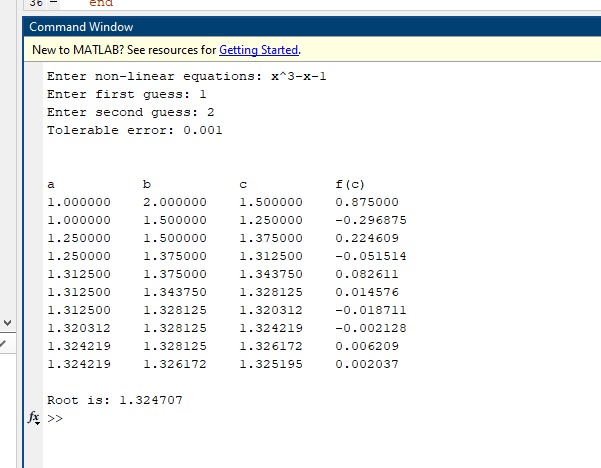
\includegraphics[width = .9\textwidth]{bisec.jpeg}
    \captionof{figure}{Bisection method}
\end{center}




\clearpage
\title{Finding root of nonlinear equation using False Position Method.}
\author{}
\date{}
\maketitle

\section*{Introduction}
\subsection*{False Position Method}
False position method is based on the fact that if $f(x)$ is real and continuous function, and for two initial guesses $a$ and $b$ brackets the root such that: $f(a)\times f(b) < 0$ then there exists at least one root between $a$ and $b$.\\\\
If $a$ and $b$ are two guesses then we compute new approximated root as:
\[c = a - \frac{f(a)\times (b-a)}{f(b) - f(a)}\]
Now we have following three different cases:
\begin{itemize}
    \item If $f(c)=0$ then the root is c.
    \item If $f(a)\times f(b)< 0$ then root lies between $a$ and $c$.
    \item If $f(a)\times f(c)> 0$ then root lies between $b$ and $c$.
\end{itemize}
And then the process is repeated until we find the root within desired accuracy.\cite{falsePos}


\section*{Tools Used}
\begin{itemize}
    \item MATLAB R2021a - for writing and running code.
    \item MacTeX -\LaTeX  compiler.
    \item VS Code with \LaTeX workshop extension as a text editor.
\end{itemize}

\section*{Process}

\subsection*{Code for False Position:}
\begin{minted}[breaklines, linenos]{matlab}
% Clearing Screen
clc
% Setting x as symbolic variable
syms x;

% Input Section
eqn = input('Enter non-linear equations: ');
a = input('Enter first guess: ');
b = input('Enter second guess: ');
e = input('Tolerable error: ');

% Finding Functional Value
fa = eval(subs(eqn,x,a));
fb = eval(subs(eqn,x,b));

% Implementing False Position Method
if fa*fb > 0 
    disp('Given initial values do not bracket the root.');
else
    c = a - (a-b) * fa/(fa-fb);
    fc = eval(subs(eqn,x,c));
    fprintf('\n\na\t\t\tb\t\t\tc\t\t\tf(c)\n');
    while abs(fc)>e
        fprintf('%f\t%f\t%f\t%f\n',a,b,c,fc);
        if fa*fc< 0
            b =c;
            fb = eval(subs(eqn,x,b));
        else
            a =c;
            fa = eval(subs(eqn,x,a));
        end
        c = a - (a-b) * fa/(fa-fb);
        fc = eval(subs(eqn,x,c));
    end
    fprintf('\nRoot is: %f\n', c);
end
\end{minted}

\subsection*{Output}
\begin{center}
    \centering
    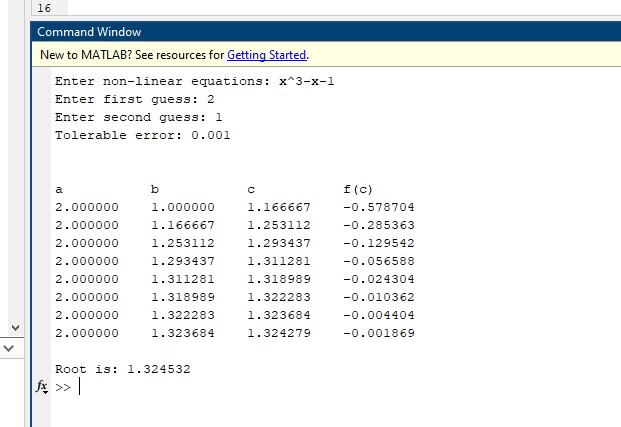
\includegraphics[width = .9\textwidth]{false.jpeg}
    \captionof{figure}{Flase Position method}
\end{center}





\clearpage
\title{Finding root of nonlinear equation using Newton-Raphson Method.}
\author{}
\date{}
\maketitle

\section*{Introduction}

\subsection*{Newton-Raphson Method}
Newton Raphson Method is an open method and starts with one initial guess for finding real root of non-linear equations.\\\\
In Newton Raphson method if $a$ is initial guess then next approximated root $b$ is obtained by following formula:
\[b = a - \frac{f(a)}{f^\prime(a)}\]
From the above equation, we get the $x$ intersect of the slope at point $(a, f(a))$. Repeating this process get this point closer and closer to real root of the non-linear equation.\cite{prs}

\section*{Tools Used}
\begin{itemize}
    \item MATLAB R2021a - for writing and running code.
    \item MacTeX -\LaTeX  compiler.
    \item VS Code with \LaTeX workshop extension as a text editor.
\end{itemize}

\section*{Process}

\subsection*{Code for Newton-Raphson:}
\begin{minted}[breaklines, linenos]{matlab}
    
% Clearing Screen
clc

% Setting x as symbolic variable
syms x;

% Input Section
eqn = input('Enter non-linear equations: ');
a = input('Enter initial guess: ');
e = input('Tolerable error: ');
N = input('Enter maximum number of steps: ');

% Initializing step counter
step = 1;

% Finding derivate of given function
g = diff(eqn,x);

% Finding Functional Value
fa = eval(subs(eqn,x,a));

while abs(fa)> e
    fa = eval(subs(eqn,x,a));
    ga = eval(subs(g,x,a));
    if ga == 0
        disp('Division by zero.');
        break;
    end
    
    b = a - fa/ga;
    fprintf('step=%d\ta=%f\tf(a)=%f\n',step,a,fa);
    a = b;
    
    if step>N
       disp('Not convergent'); 
       break;
    end
    step = step + 1;
end

fprintf('Root is %f\n', a);
\end{minted}



\vspace{20mm}
\subsection*{Output}
\begin{center}
    \centering
    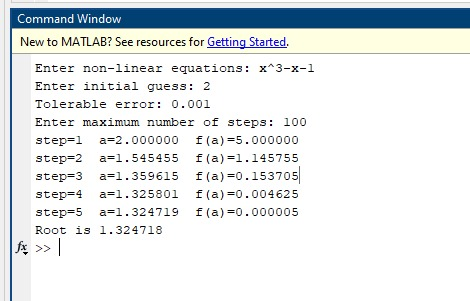
\includegraphics[width = .9\textwidth]{newar.jpeg}
    \captionof{figure}{Newton-Raphson method}
\end{center}


\pagebreak
\section*{Functions}
The functions used to do the three methods in MATLAB are as such with brief description of each of them:
\begin{description}
    \item[syms] Create symbolic scalar variables and functions, and matrix variables and functions. By using $syms\;\;x$, a variable $x$ is declared for the the code. So anywhere in the code input, if there is x, it can be accessed as a variable.
    \item[input()] $x\;=\;input(prompt)$ displays the text in prompt and waits for the user to input a value and press the Return key. The user can enter expressions, like $pi/4$ or $rand(3)$, and can use variables in the workspace.
    \item[eval()] Evaluates a MATLAB expressions.
    \item[subs()] Symbolic substitution. subs(s,new) returns a copy of $s$, replacing all occurrences of the symbolic scalar variable (declared as $syms\;x$) in $s$ with $new$ ($new$ can be a number or another variable), and then evaluates $s$.
    \item[disp()] $disp(X)$ displays the value of variable $X$ without printing the variable name.
    \item[fprintf()] Like the $printf()$ function in C language. Unline $disp()$ using this function data can be written in text.
    \item[if\_else] $if\;expression$, $statements$, $end$ evaluates an expression, and executes a group of statements when the expression is true. An expression is true when its result is nonempty and contains only nonzero elements (logical or real numeric). Otherwise, the expression is false.\\
          The $elseif$ and $else$ blocks are optional. The statements execute only if previous expressions in the $if...\;end$ block are false. An if block can include multiple elseif blocks.
    \item[while] $while\;expression$, $statements$, $end$ evaluates an expression, and repeats the execution of a group of statements in a loop while the expression is true. An expression is true when its result is nonempty and contains only nonzero elements (logical or real numeric). Otherwise, the expression is false.
\end{description}
These function are the newly learned ones for these experiments.\cite{matlab}
\pagebreak
\bibliographystyle{IEEEtran}
\bibliography{ref}

\end{document}
